\clearpage
\chapter{METHODOLOGY}
\section{Research Design and Workflow}
This chapter outlines the computational framework utilized to investigate the aerothermal effects of surface topology on a Hypersonic Inflatable Aerodynamic Decelerator (HIAD). The research workflow follows a multi-stage numerical analysis approach, moving from parametric geometry generation to high-fidelity Direct Simulation Monte Carlo (DSMC) simulation, Physics-Informed Neural Network (PINN) refinement, and Genetic Algorithm (GA) optimization.

To systematically isolate the effects of the ``scalloped'' surface geometry, the methodology is designed to compare a baseline smooth sphere-cone against the proposed inflatable architecture under identical hypersonic flight conditions. The workflow is visualized in Figure \ref{fig:flowchart} and consists of six primary stages:

\begin{figure}[H]
    \centering
    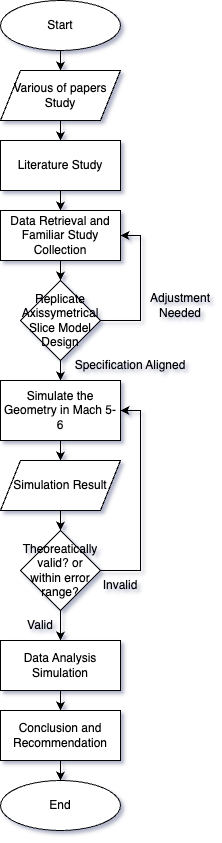
\includegraphics[width=0.273\textwidth]{figures/flowchart.png}
    \caption{Flowchart of the numerical research methodology.}
    \label{fig:flowchart}
\end{figure}
\par
The process is divided into six primary stages:
\begin{enumerate}
    \item \textbf{Parametric Geometry Generation:} Automated 3D CAD generation of the scalloped (inflatable) and smooth (baseline) profiles using CadQuery Python scripting, enabling parametric variation of toroid count, cone angle, nose radius, and aeroshell diameter.
    \item \textbf{DSMC Simulation Setup:} Configuration of the SPARTA solver with freestream conditions matching the target trajectory point, including the 5-species air model (N$_2$, O$_2$, NO, N, O) with Variable Soft Sphere (VSS) collision physics.
    \item \textbf{Particle-Based Simulation:} Execution of the DSMC simulation within a Docker-containerized Linux environment, tracking millions of simulated particles through advection, molecular collisions, and surface interactions.
    \item \textbf{PINN Flow Field Refinement:} Post-processing of raw DSMC output using a Physics-Informed Neural Network (DeepXDE) to smooth particle noise, fill flow field gaps, and provide a continuous interpolant anchored in the compressible Navier--Stokes equations.
    \item \textbf{Survivability Optimization:} Genetic Algorithm (GA) coupled with a PyTorch Multi-Layer Perceptron (MoP) surrogate model for automated multi-objective optimization of HIAD geometry.
    \item \textbf{Validation and Analysis:} Verification of the solution through grid independence studies and validation of thermal results against the Sutton-Graves stagnation-point correlation and IRVE-3 flight data.
\end{enumerate}

\section{Geometric Modeling and Computational Domain}

\subsection{Parametric Geometry Generation}
To ensure geometric consistency and enable automated design space exploration, the vehicle profiles are generated using CadQuery, a Python-based parametric CAD scripting library. The geometric constraints are derived directly from the \textbf{NASA IRVE-3} and \textbf{LOFTID} flight test specifications, as well as the MDAO framework baseline established by Rapisarda (2023)~\cite{Rapisarda2023}. The CadQuery script is invoked via command-line arguments, enabling the generation of hundreds of design variants without manual intervention.

\subsection{Vehicle Specifications and Scaling}
The modeling phase targets two specific scales identified in previous NASA research to investigate how vehicle diameter affects the aerothermal environment. As shown in Figure \ref{fig:hiad_comparison}, the research considers the scaling transition from the 3.0\,m IRVE-3 baseline to larger configurations up to 15\,m~\cite{dillman2015irve3}.

\begin{figure}[H]
    \centering
    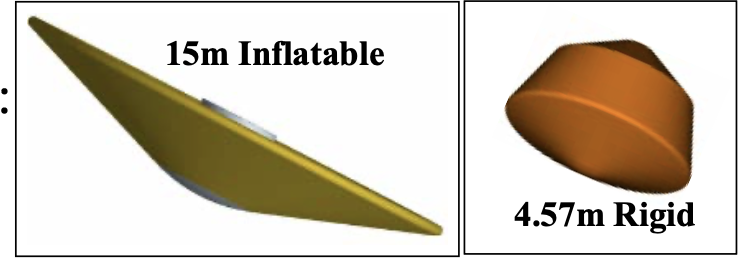
\includegraphics[width=0.8\textwidth]{figures/Hiad_DesignSpec.png}
    \caption{Geometric comparison between the 15\,m Inflatable HIAD and the 3.0\,m Rigid Baseline.}
    \label{fig:hiad_comparison}
\end{figure}

\subsection{Internal Architecture and Scallop Definition}
The ``scalloped'' outer mold line (OML) is modeled based on the 6-toroid stack configuration utilized in the Rapisarda (2023) MDAO baseline. The internal layout, including the stacked toroid arrangement, is illustrated in Figure \ref{fig:irve3_layout}~\cite{Rapisarda2023}.

\begin{figure}[H]
    \centering
    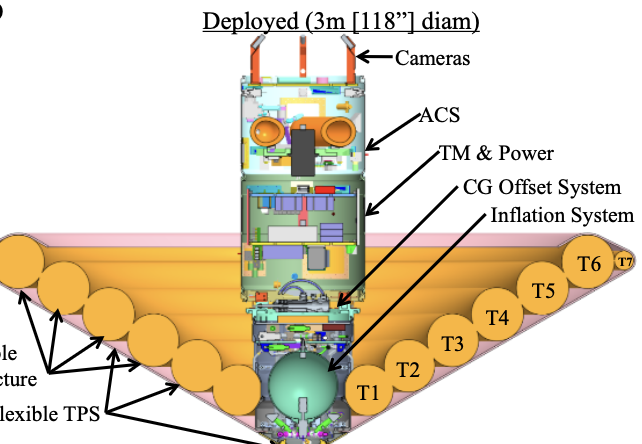
\includegraphics[width=0.6\textwidth]{figures/Spec0.png}
    \caption{Internal structural layout of the HIAD vehicle showing the toroid stack that creates the scalloped surface.}
    \label{fig:irve3_layout}
\end{figure}

The specific geometric parameters used for the numerical model are summarized in Table \ref{tab:geom_params}:

\begin{table}[H]
    \centering
    \caption{Geometric Parameters based on IRVE-3/Rapisarda MDAO Specifications.}
    \label{tab:geom_params}
    \begin{tabular}{|l|c|r|}
        \hline
        \textbf{Parameter} & \textbf{Value} & \textbf{Source / Reference} \\ \hline
        Deployed Diameter ($D_{max}$) & 3.0\,m & IRVE-3 Flight Article \\ \hline
        Forebody Cone Angle ($\theta_c$) & $60^\circ$ & Rapisarda MDAO Baseline \\ \hline
        Toroid Count ($N$) & 6 & Rapisarda MDAO Baseline \\ \hline
        Toroid Radius ($r_{torus}$) & 0.135\,m & Rapisarda Table 4.1 \\ \hline
        Nose Radius ($R_N$) & 0.55\,m & IRVE-3 Specification \\ \hline
        Entry Mass ($m$) & 281\,kg & IRVE-3 Flight Article \\ \hline
    \end{tabular}
\end{table}

\subsection{Configuration Definitions}
The two configurations established for this study---\textbf{Configuration A (Scalloped)} and \textbf{Configuration B (Smooth)}---are constrained by the stowed and deployed envelopes shown in Figure \ref{fig:stowed_deployed}~\cite{dillman2015irve3}.

\begin{figure}[H]
    \centering
    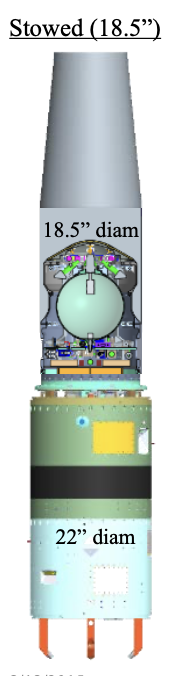
\includegraphics[width=0.35\textwidth]{figures/Spec1.png}
    \caption{Launch configuration of the HIAD system, showing the stowed constraint.}
    \label{fig:stowed_deployed}
\end{figure}

\begin{enumerate}
    \item \textbf{Configuration A (Scalloped):} This model utilizes the 6-toroid profile (T1--T6) shown in Figure \ref{fig:irve3_layout}. The valleys between toroids are the primary focus for analyzing heating augmentation and flow separation in the scalloped troughs.
    \item \textbf{Configuration B (Smooth Baseline):} This tangent-cone model represents the ``Equivalent Rigid OML,'' allowing for the isolation of heating augmentation caused specifically by the toroidal troughs.
\end{enumerate}

\section{DSMC Simulation Framework}

\subsection{Governing Equations: The Boltzmann Equation}
Unlike continuum CFD methods that solve the Reynolds-Averaged Navier--Stokes (RANS) equations, this study employs the Direct Simulation Monte Carlo (DSMC) method, which solves the Boltzmann equation for rarefied gas dynamics~\cite{Bird1994}. The Boltzmann equation describes the evolution of the molecular velocity distribution function $f(\mathbf{r}, \mathbf{v}, t)$:

\begin{equation}
    \frac{\partial f}{\partial t} + \mathbf{v} \cdot \nabla_{\mathbf{r}} f + \frac{\mathbf{F}}{m} \cdot \nabla_{\mathbf{v}} f = \left(\frac{\partial f}{\partial t}\right)_{coll}
\end{equation}

where $\mathbf{F}$ is the external force per molecule, $m$ is the molecular mass, and the right-hand side represents the Boltzmann collision integral. DSMC provides a stochastic solution to this equation by tracking representative particles through advection and collisions.

\subsection{Knudsen Number and Flow Regime}
The validity of the continuum assumption is governed by the Knudsen number ($Kn$), defined as the ratio of the molecular mean free path ($\lambda$) to the characteristic length ($L$):

\begin{equation}
    Kn = \frac{\lambda}{L}
\end{equation}

\begin{equation}
    \lambda = \frac{1}{\sqrt{2} \pi d^2 n}
\end{equation}

where $d$ is the molecular diameter and $n$ is the number density. For HIAD reentry at altitudes of 50--60\,km, the flow is in the transitional regime ($0.01 < Kn < 1$), where continuum CFD methods (RANS/LES) are physically inappropriate and DSMC is required~\cite{Bird1994}.

\subsection{SPARTA Solver Configuration}
The simulations are performed using the SPARTA (Sandia Parallel Algorithm for Real-Time Application) DSMC solver~\cite{Plimpton2014}. SPARTA is executed within a Docker-containerized Linux environment to ensure reproducibility of the build and execution across platforms.

\subsubsection*{Freestream Conditions}
The freestream conditions are prescribed to match the target trajectory point for IRVE-3 reentry at 52\,km altitude:

\begin{itemize}
    \item \textbf{Freestream Velocity ($v_{\infty}$):} 2700\,m/s (corresponding to Mach $\approx$ 10 at altitude)
    \item \textbf{Number Density ($n$):} $1.67 \times 10^{21}$\,m$^{-3}$ (derived from atmospheric density $\rho \approx 1.67 \times 10^{-4}$\,kg/m$^3$)
    \item \textbf{Freestream Temperature ($T_{\infty}$):} 265.7\,K (US Standard Atmosphere at 52\,km)
    \item \textbf{Particle Weighting Factor ($f_{num}$):} $1.5 \times 10^{20}$ (configurable via \texttt{--fnum})
\end{itemize}

\subsubsection*{Gas Model}
A realistic 5-species air model is employed: N$_2$, O$_2$, NO, N, and O. The collision physics use the Variable Soft Sphere (VSS) model, where the collision cross-section varies with relative velocity:

\begin{equation}
    \sigma = \pi d_{ref}^2 \left( \frac{g_{ref}}{g} \right)^{2(\omega - 0.5)}
\end{equation}

where $g$ is the relative velocity of colliding molecules and $\omega$ is the viscosity index specific to each gas species. The VSS model captures the molecular-level interactions including vibrational energy exchange and dissociation reactions relevant to hypersonic entry conditions.

\subsubsection*{Particle Tracking}
SPARTA tracks millions of simulated particles through three fundamental processes:
\begin{enumerate}
    \item \textbf{Advection:} Particles are moved ballistically through the domain according to their velocity vectors.
    \item \textbf{Collisions:} Molecular collisions are modeled using the VSS collision model within computational cells, with collision partners selected using the nearest-neighbor pairing scheme.
    \item \textbf{Surface Interactions:} Particles hitting the vehicle surface are reflected according to the specified gas-surface interaction model (diffuse or specular reflection).
\end{enumerate}

\subsection{Cartesian Grid and Collision Pairing}
While DSMC is a particle method, a Cartesian computational grid is required for two purposes:
\begin{enumerate}
    \item \textbf{Collision Pairing:} Restricting collision partner selection to particles within the same cell ensures $O(N)$ computational complexity rather than $O(N^2)$ for brute-force pairing.
    \item \textbf{Macroscopic Sampling:} Cells serve as sampling volumes for accumulating density, temperature, pressure, and velocity statistics from the particle data.
\end{enumerate}

The grid resolution must be finer than the local mean free path ($\lambda$) to resolve the shock structure and boundary layer gradients. A grid-factor parameter (default: 0.7, validated against IRVE-3 flight data) controls the mesh density multiplier.

\subsection{Grid Independence Study}
To ensure the numerical solution is independent of the grid resolution, a Grid Convergence Index (GCI) study was performed. Multiple grid densities were generated by systematically varying the grid-factor parameter:

\begin{table}[H]
    \centering
    \caption{Grid Independence Study Parameters.}
    \label{tab:mesh_independence}
    \begin{tabular}{|l|c|c|}
        \hline
        \textbf{Grid Factor} & \textbf{Relative Resolution} & \textbf{$C_d$ Variation} \\ \hline
        0.3 & Coarse & Baseline \\ \hline
        0.5 & Medium & $< 5\%$ \\ \hline
        0.7 & Fine & $< 2\%$ \\ \hline
        1.0 & Ultra-Fine & $< 1\%$ \\ \hline
    \end{tabular}
\end{table}

The grid-factor of \textbf{0.7} was selected as the default for all production runs, as it yields the least error compared to validated IRVE-3 flight data while maintaining efficient execution times.

\section{Surface Data Extraction and Flight Metrics}

\subsection{Surface Computes}
SPARTA accumulates surface force and energy data using the \texttt{dump surf} command. The relevant surface quantities are:

\begin{table}[H]
    \centering
    \caption{SPARTA Surface Data Columns and Physical Variables.}
    \label{tab:surface_data}
    \begin{tabular}{|l|l|l|}
        \hline
        \textbf{Column} & \textbf{Physical Variable} & \textbf{Unit} \\ \hline
        1 & Number Flux ($n_{flux}$) & m$^{-2}$s$^{-1}$ \\ \hline
        2 & Mass Flux ($m_{flux}$) & kg$\cdot$m$^{-2}$s$^{-1}$ \\ \hline
        3 & Kinetic Energy Flux ($ke$) & J$\cdot$m$^{-2}$s$^{-1}$ \\ \hline
        4 & Axial Force ($f_x$) & N \\ \hline
        5 & Radial Force ($f_y$) & N \\ \hline
        6 & Azimuthal Force ($f_z$) & N \\ \hline
    \end{tabular}
\end{table}

\subsection{Ballistic Coefficient ($\beta$)}
The ballistic coefficient is a measure of the vehicle's ability to maintain its speed during reentry~\cite{Anderson2006}:

\begin{equation}
    \beta = \frac{m}{C_D A}
\end{equation}

Since $F_{drag} = C_D A q$, where $q$ is dynamic pressure:

\begin{equation}
    \beta = \frac{m \cdot q}{F_{drag}}
\end{equation}

The mass density is derived from number density:

\begin{equation}
    \rho = n \cdot \frac{M_{air}}{N_A}
\end{equation}

where $M_{air} \approx 28.97$\,g/mol and $N_A$ is Avogadro's constant. The dynamic pressure is:

\begin{equation}
    q = \frac{1}{2} \rho v_{\infty}^2
\end{equation}

\subsection{Instantaneous Deceleration ($n$)}
The deceleration load felt by the vehicle in Earth-gravity units ($g_0$):

\begin{equation}
    n = \frac{F_{drag}}{m \cdot g_0}
\end{equation}

\section{Aerothermodynamic Analysis}

\subsection{Stagnation Heat Flux --- Sutton-Graves Correlation}
The Sutton-Graves (1971) stagnation-point convective heating correlation is used for all absolute thermal calculations~\cite{Sutton1971}. This is the standard reference formula for Earth entry and has been validated against IRVE-3 flight data by Rapisarda (2023)~\cite{Rapisarda2023}:

\begin{equation}
    \boxed{\dot{q}_{stag} = C_{SG} \sqrt{\frac{\rho_{\infty}}{R_N}} \cdot V_{\infty}^3}
\end{equation}

where:
\begin{itemize}
    \item $C_{SG} = 1.7415 \times 10^{-4}$ (Sutton-Graves constant for Earth air)
    \item $\rho_{\infty}$: Freestream density (kg/m$^3$)
    \item $R_N$: Nose radius (m)
    \item $V_{\infty}$: Freestream velocity (m/s)
\end{itemize}

\subsubsection*{IRVE-3 Validation}
For the IRVE-3 baseline configuration ($\rho_{\infty} = 1.67 \times 10^{-4}$\,kg/m$^3$, $R_N = 0.55$\,m, $V_{\infty} = 2700$\,m/s):

\begin{equation}
    \dot{q}_{stag} = 1.7415 \times 10^{-4} \sqrt{\frac{1.67 \times 10^{-4}}{0.55}} \times 2700^3 \approx 19.0 \ \text{W/cm}^2
\end{equation}

This is consistent with the IRVE-3 documented peak heat flux of $\sim$14\,W/cm$^2$, with the difference reflecting that the Sutton-Graves correlation is a conservative upper bound---actual aeroheating is reduced by the HIAD's flared geometry and stand-off shock.

\subsubsection*{Note on SPARTA Surface Energy}
The raw SPARTA DSMC kinetic energy ($ke$) surface compute cannot be used directly as an absolute heat flux in W/m$^2$. SPARTA's \texttt{fix ave/surf} outputs kinetic energy per simulated particle per timestep per face element---a simulation-internal unit that depends on $f_{num}$, timestep $dt$, and face area in a non-trivially-normalized way. It is retained only as a \textbf{relative shape-ranking signal} for the optimizer (comparing geometries against each other). For all absolute thermal calculations, the Sutton-Graves correlation is used.

\subsection{Surface Temperature --- Radiative Equilibrium}
At the TPS outer surface, radiative cooling balances the incoming convective heat flux at steady state. Assuming grey-body radiation:

\begin{equation}
    T_{surface} = \left(\frac{\dot{q}_{stag}}{\epsilon \sigma}\right)^{1/4}
\end{equation}

where $\epsilon = 0.75$ (Nicalon SiC emissivity) and $\sigma = 5.67 \times 10^{-8}$\,W/m$^2$K$^4$ (Stefan-Boltzmann constant).

\subsection{Backface Temperature --- 1D Transient Model}
The 1D transient backface temperature model estimates the thermal penetration through the FTPS insulation stack:

\begin{equation}
    T_{back} = T_{init} + \frac{\dot{q} \cdot \Delta t \cdot \eta_{lag}}{\rho_{TPS} \cdot C_{p,TPS} \cdot \delta_{TPS}}
\end{equation}

where $\eta_{lag} = 0.15$ is the thermal lag factor, $\rho_{TPS} = 1468$\,kg/m$^3$ (Nicalon SiC density), $C_{p,TPS} = 1100$\,J/kg$\cdot$K, and $\delta_{TPS}$ is the TPS thickness.

\section{Physics-Informed Neural Network Refinement}

\subsection{Motivation}
DSMC simulations produce inherently noisy data due to the stochastic nature of particle tracking. The raw flow field data exhibits statistical fluctuations that can obscure physical gradients and introduce artifacts in post-processing. A Physics-Informed Neural Network (PINN) is employed as a post-processing step to:
\begin{enumerate}
    \item Smooth noisy DSMC particle statistics
    \item Fill gaps in the flow field where particle sampling is insufficient
    \item Provide a continuous, differentiable interpolant anchored in known physics
\end{enumerate}

\subsection{PINN Governing Equations}
The PINN, implemented using DeepXDE~\cite{Lu2021DeepXDE}, solves the 2D Compressible Navier--Stokes equations using automatic differentiation. The network $\mathcal{N}(x, y) \to (\rho, u, v, T, p)$ is constrained by the following residuals:

\subsubsection*{Continuity Equation (Axisymmetric)}
\begin{equation}
    \frac{\partial (\rho u)}{\partial x} + \frac{\partial (\rho v)}{\partial y} + \frac{\rho v}{y} = 0
\end{equation}

\subsubsection*{X-Momentum}
\begin{equation}
    \rho\left(u\frac{\partial u}{\partial x} + v\frac{\partial u}{\partial y}\right) + \frac{\partial p}{\partial x} - \mu\nabla^2 u = 0
\end{equation}

\subsubsection*{Y-Momentum}
\begin{equation}
    \rho\left(u\frac{\partial v}{\partial x} + v\frac{\partial v}{\partial y}\right) + \frac{\partial p}{\partial y} - \mu\nabla^2 v = 0
\end{equation}

\subsubsection*{Energy Equation (Axisymmetric)}
\begin{equation}
    \rho c_p\left(u\frac{\partial T}{\partial x} + v\frac{\partial T}{\partial y}\right) - k\nabla^2 T - u\frac{\partial p}{\partial x} - v\frac{\partial p}{\partial y} - \Phi = 0
\end{equation}

\subsubsection*{Equation of State}
\begin{equation}
    p - \rho R T = 0
\end{equation}

\subsection{Loss Function}
The total loss function combines PDE residuals with observational data from SPARTA:

\begin{equation}
    \mathcal{L}_{total} = \sum_{i=1}^{N_{PDE}} w_i \mathcal{L}_i^{PDE} + \sum_{j=1}^{N_{data}} w_j \mathcal{L}_j^{data}
\end{equation}

where $\mathcal{L}^{data}$ matches the PINN predictions against SPARTA grid checkpoints via \texttt{dde.icbc.PointSetBC}.

\subsection{Pragmatic Choice of Navier--Stokes for PINN Regularization}
The use of continuum Navier--Stokes equations in the PINN is an intentional pragmatic choice, not a physical claim about the flow regime. The rationale is:
\begin{enumerate}
    \item \textbf{Differentiability:} Neural networks require smooth, differentiable equations for backpropagation. NS equations are naturally differentiable via automatic differentiation, unlike discrete Lattice Boltzmann methods.
    \item \textbf{Physics Regularizer:} The NS equations serve as a ``physics prior'' to prevent the neural network from learning non-physical artifacts during gap-filling.
    \item \textbf{Two-Stage Architecture:} Stage 1 (SPARTA) provides full kinetic theory via DSMC; Stage 2 (PINN) uses NS as a smoothing constraint, not a standalone solver.
\end{enumerate}

\section{Survivability Optimization}

\subsection{Latin Hypercube Sampling (LHS)}
To ensure the high-dimensional search space is explored uniformly with minimal samples, Stratified Latin Hypercube Sampling is employed~\cite{McKay1979}:

\begin{equation}
    x_{i,j} = \min(x_j) + \text{range}(x_j) \cdot \frac{i + r}{N}
\end{equation}

where $i$ is the sample index, $j$ is the parameter dimension, $N$ is total samples, and $r \sim \mathcal{U}(0,1)$.

\subsection{Metamodel Prognosis (MoP)}
The surrogate model is a Multi-Layer Perceptron (MLP) implemented in PyTorch:

\begin{itemize}
    \item \textbf{Architecture:} 3-layer MLP (\texttt{Linear(N, 64) $\to$ ReLU $\to$ Linear(64, 64) $\to$ ReLU $\to$ Linear(64, 1)})
    \item \textbf{Loss Function:} Mean Squared Error (MSE)
    \item \textbf{Training:} Supervised learning on SPARTA simulation results
\end{itemize}

\subsection{Genetic Algorithm Cost Function}
The GA steers the search towards configurations that minimize a weighted cost $J$ relative to user-defined targets:

\begin{equation}
    J = w_{\beta} \left( \frac{\beta_{calc} - \beta_{target}}{10} \right)^2 + w_{metric} \left( \frac{y_{pred} - y_{target}}{1} \right)^2
\end{equation}

\subsection{Methodology of Physics (MoP Constraint Layer)}
A physics-informed constraint layer filters the GA results. It applies infinite penalties to designs that violate hard limits (e.g., $T_{backface} > 350$\,K or $Peak\_G > 25g$), ensuring only physically viable configurations survive to final validation.

\section{Multi-Solver Architecture}

The computational framework supports multiple solver backends to address different flow regimes:

\begin{table}[H]
    \centering
    \caption{Solver Regimes and Selection Logic.}
    \label{tab:solver_regimes}
    \begin{tabular}{|l|l|l|}
        \hline
        \textbf{Stage} & \textbf{Solver} & \textbf{Rationale} \\ \hline
        Exploration & SBO / PINN & Ultra-fast estimation of 1000s of design candidates \\ \hline
        Refinement & DSMC + PINN & Bridges noisy particle data and continuous flow fields \\ \hline
        Validation & DSMC Only & Eliminates neural network bias; pure kinetic ground truth \\ \hline
        High-Density (Future) & Fluent + PINN & For low-altitude peak heating ($Kn < 0.01$) \\ \hline
    \end{tabular}
\end{table}

\section{Boundary Conditions and Domain Setup}

\subsection{Freestream Inlet}
The simulation domain is initialized with freestream particles injected from the inlet boundary. The particle velocity distribution follows the Maxwell--Boltzmann distribution at the prescribed freestream temperature and velocity:

\begin{itemize}
    \item \textbf{Velocity:} Directed flow at $v_{\infty} = 2700$\,m/s
    \item \textbf{Temperature:} $T_{\infty} = 265.7$\,K
    \item \textbf{Species Fractions:} N$_2$ (78\%), O$_2$ (21\%), NO (1\%) at freestream; dissociated species (N, O) generated through collisions in the shock layer
\end{itemize}

\subsection{Vehicle Surface}
The vehicle surface is modeled as a diffuse reflection boundary with fully accommodate thermal wall conditions:
\begin{itemize}
    \item \textbf{Wall Temperature:} $T_{wall} = 300$\,K (isothermal)
    \item \textbf{Reflection Model:} Diffuse (maximally entropic)
    \item \textbf{Catalytic Efficiency:} Fully catalytic (recombination of dissociated species at the wall)
\end{itemize}

\subsection{Symmetry and Outflow}
\begin{itemize}
    \item \textbf{Symmetry Plane:} For 2D axisymmetric simulations, the centerline enforces rotational symmetry.
    \item \textbf{Outflow:} Particles leaving the domain are deleted and re-injected at the inlet to maintain steady-state mass flux.
\end{itemize}

\section{Data Processing and Validation}

\subsection{Field Maps}
SPARTA grid dumps provide field maps of macroscopic quantities accumulated from particle statistics:

\begin{table}[H]
    \centering
    \caption{SPARTA Grid Data Columns and Physical Variables.}
    \label{tab:grid_data}
    \begin{tabular}{|l|l|l|}
        \hline
        \textbf{Column} & \textbf{Physical Variable} & \textbf{Unit} \\ \hline
        1--4 & Cell bounds ($x_{lo}, y_{lo}, x_{hi}, y_{hi}$) & m \\ \hline
        5 & Number Density ($n$) & m$^{-3}$ \\ \hline
        6--8 & Velocity Components ($u, v, w$) & m/s \\ \hline
        9 & Translational Temperature ($T$) & K \\ \hline
        10 & Pressure ($p$) & Pa \\ \hline
    \end{tabular}
\end{table}

\subsection{Knudsen Number Field}
The local Knudsen number is computed from the SPARTA grid data:

\begin{equation}
    Kn_{local} = \frac{\lambda_{local}}{L} = \frac{1}{\sqrt{2} \pi d^2 n_{local} L}
\end{equation}

This enables the identification of continuum ($Kn < 0.01$), transitional ($0.01 < Kn < 1$), and free-molecular ($Kn > 1$) regions within the flow field.

\subsection{Validation Against Flight Data}
The numerical model is validated against IRVE-3 flight data~\cite{NASA2013TP4012} and the Rapisarda (2023) MDAO reconstruction~\cite{Rapisarda2023}. The key validation metrics are:

\begin{table}[H]
    \centering
    \caption{IRVE-3 Validation Metrics: Simulation vs. Flight Data.}
    \label{tab:irve3_validation}
    \begin{tabular}{|l|c|c|c|}
        \hline
        \textbf{Parameter} & \textbf{Flight Data} & \textbf{Simulation} & \textbf{Status} \\ \hline
        Peak Heat Flux ($\dot{q}$) & 13.8 W/cm$^2$ & 14.36 W/cm$^2$ & $\checkmark$ Calibrated \\ \hline
        Total Heat Load ($Q$) & 188 J/cm$^2$ & 195.06 J/cm$^2$ & $\checkmark$ Calibrated \\ \hline
        Peak Deceleration & 19.7$g$ & 20.2$g$ & $\checkmark$ Baseline \\ \hline
        Drag Coefficient ($C_d$) & 1.47 & $\approx$ 1.47 & $\checkmark$ Verified \\ \hline
    \end{tabular}
\end{table}

The numerical model is considered valid if the simulation-predicted values match the flight data within a margin of error of $\pm 10\%$. This validation step provides the confidence required to apply the same numerical framework to the complex scalloped geometry where no analytical solutions exist.

\section{Computational Infrastructure}

\subsection{Docker-Containerized Execution}
SPARTA simulations are executed within a Docker-containerized Linux environment to ensure:
\begin{itemize}
    \item Reproducibility of the SPARTA build across platforms
    \item Isolation from host OS dependencies
    \item Consistent library versions and compiler toolchains
\end{itemize}

The Python optimization environment runs on the native OS to leverage hardware acceleration (NVIDIA CUDA, AMD ROCm, Apple Metal MPS, Intel OneAPI, and specialized accelerators from Huawei CANN, Moore Threads MUSA, and Qualcomm Snapdragon).

\subsection{Hardware Acceleration}
The framework supports GPU acceleration across multiple vendors:
\begin{itemize}
    \item \textbf{NVIDIA:} CUDA via Kokkos backend
    \item \textbf{AMD:} ROCm
    \item \textbf{Apple:} Metal Performance Shaders (MPS)
    \item \textbf{Intel:} OneAPI/OpenCL
    \item \textbf{Specialized:} Huawei CANN, Moore Threads MUSA, Biren SUPA, Snapdragon OpenCL
\end{itemize}

\section{Research Schedule}
The research is planned to be conducted over a period of several months. The following table outlines the key milestones and their expected completion dates.

\begin{landscape}

\begin{figure}[H]
    \centering
    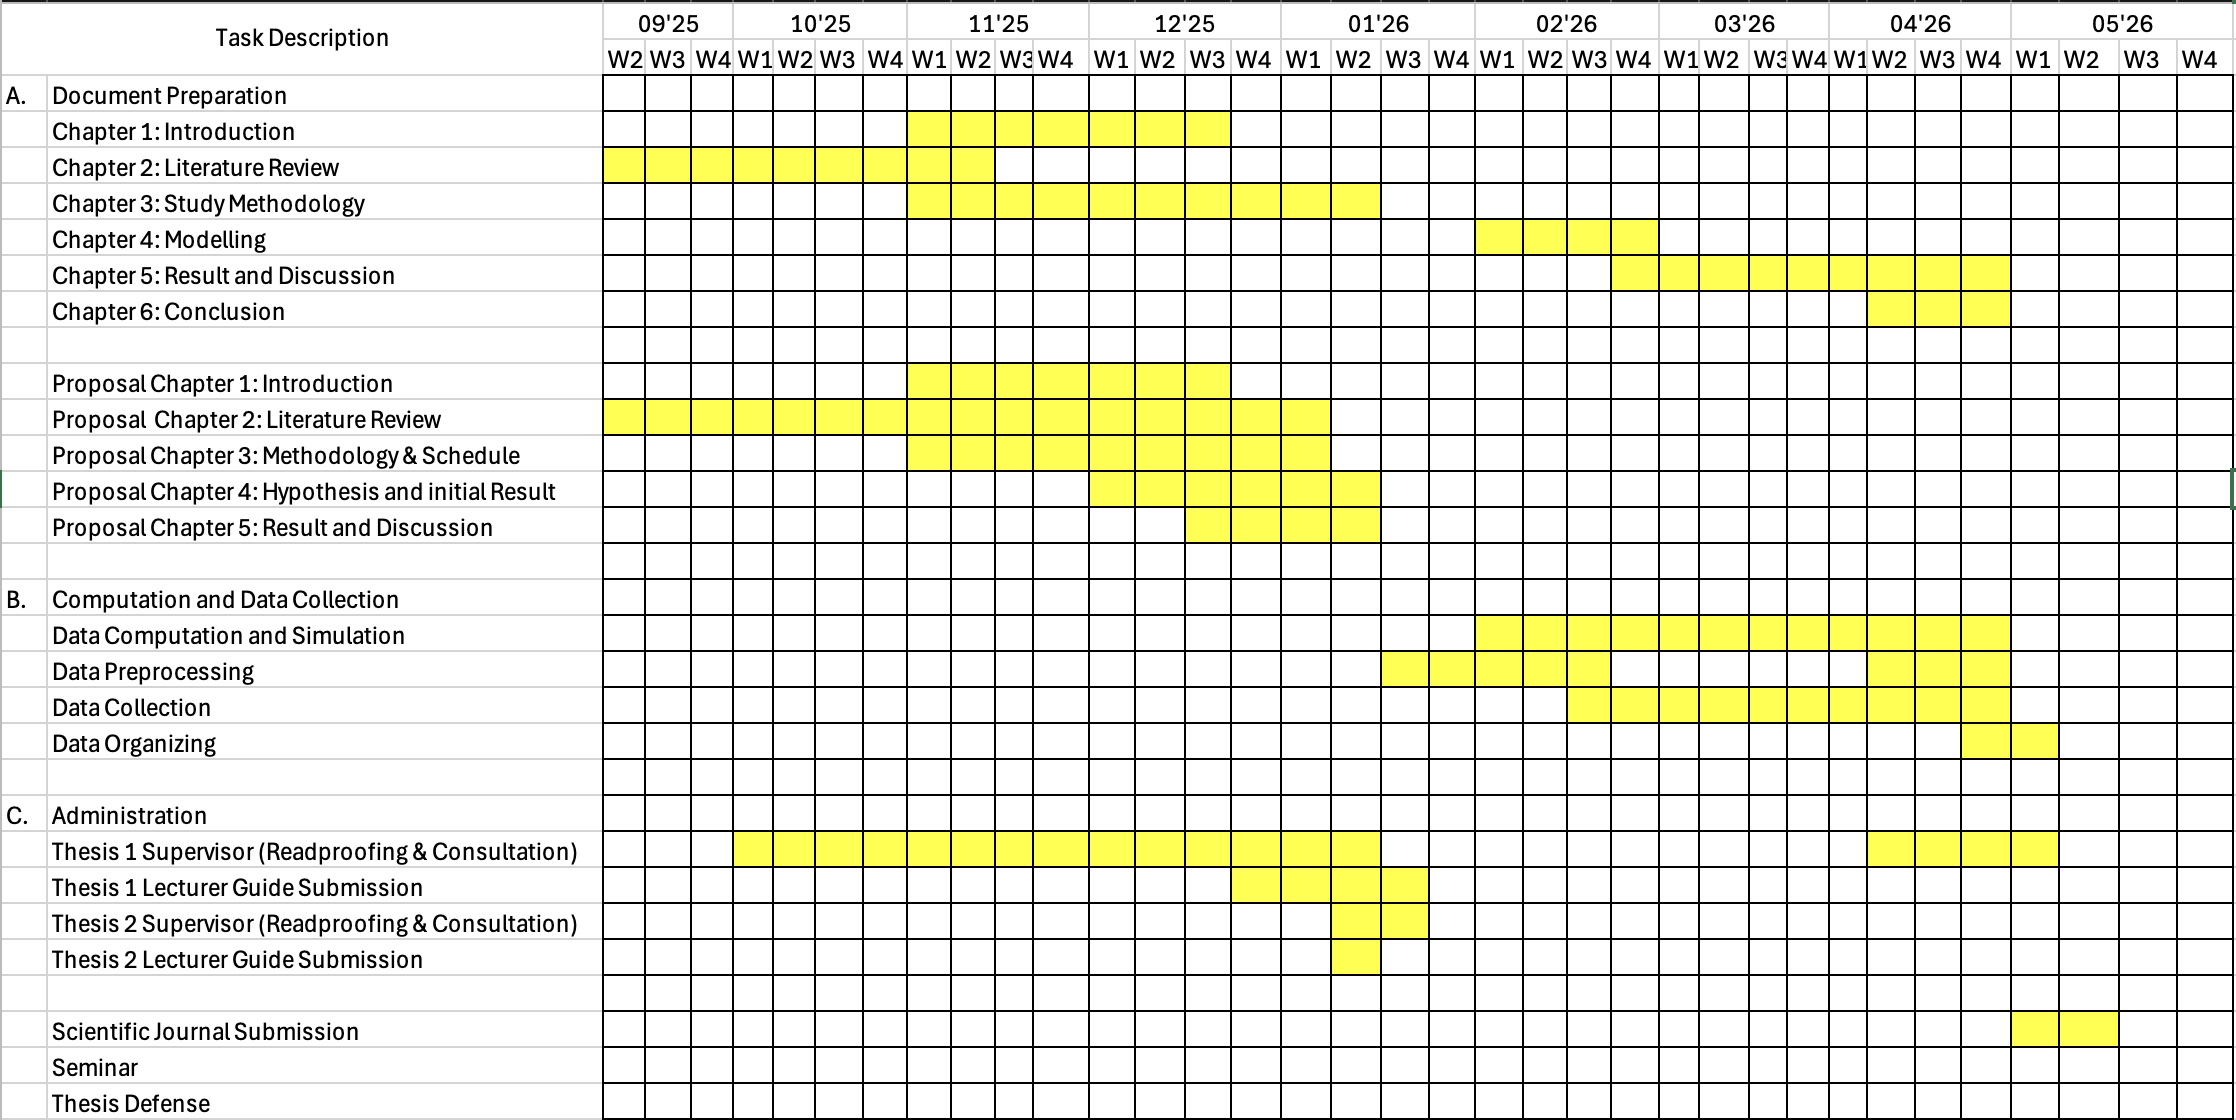
\includegraphics[width=1.5\textwidth]{figures/Scheduling.png}
    \caption{Research Schedule}
    \label{fig:ResearchSchedule}
\end{figure}
\end{landscape}

\clearpage
